% This is "sig-alternate.tex" V2.1 April 2013
% This file should be compiled with V2.5 of "sig-alternate.cls" May 2012
%
% This example file demonstrates the use of the 'sig-alternate.cls'
% V2.5 LaTeX2e document class file. It is for those submitting
% articles to ACM Conference Proceedings WHO DO NOT WISH TO
% STRICTLY ADHERE TO THE SIGS (PUBS-BOARD-ENDORSED) STYLE.
% The 'sig-alternate.cls' file will produce a similar-looking,
% albeit, 'tighter' paper resulting in, invariably, fewer pages.
%
% ----------------------------------------------------------------------------------------------------------------
% This .tex file (and associated .cls V2.5) produces:
%       1) The Permission Statement
%       2) The Conference (location) Info information
%       3) The Copyright Line with ACM data
%       4) NO page numbers
%
% as against the acm_proc_article-sp.cls file which
% DOES NOT produce 1) thru' 3) above.
%
% Using 'sig-alternate.cls' you have control, however, from within
% the source .tex file, over both the CopyrightYear
% (defaulted to 200X) and the ACM Copyright Data
% (defaulted to X-XXXXX-XX-X/XX/XX).
% e.g.
% \CopyrightYear{2007} will cause 2007 to appear in the copyright line.
% \crdata{0-12345-67-8/90/12} will cause 0-12345-67-8/90/12 to appear in the copyright line.
%
% ---------------------------------------------------------------------------------------------------------------
% This .tex source is an example which *does* use
% the .bib file (from which the .bbl file % is produced).
% REMEMBER HOWEVER: After having produced the .bbl file,
% and prior to final submission, you *NEED* to 'insert'
% your .bbl file into your source .tex file so as to provide
% ONE 'self-contained' source file.
%
% ================= IF YOU HAVE QUESTIONS =======================
% Questions regarding the SIGS styles, SIGS policies and
% procedures, Conferences etc. should be sent to
% Adrienne Griscti (griscti@acm.org)
%
% Technical questions _only_ to
% Gerald Murray (murray@hq.acm.org)
% ===============================================================
%
% For tracking purposes - this is V2.0 - May 2012

%\newif\ifdraft
%\drafttrue
%\draftfalse


\documentclass{sig-alternate-05-2015}
\usepackage{url}
\usepackage{epsfig}
\usepackage{makeidx}         % allows index generation
\usepackage{graphicx}        % standard LaTeX graphics tool
                             % when including figure files
\usepackage{multicol}        % used for the two-column index
\usepackage[bottom]{footmisc}% places footnotes at page bottom
\usepackage{float}           % H para posicionar figuras
\usepackage{booktabs}
\usepackage[usenames,dvipsnames]{xcolor}
\usepackage{xspace}


\ifdraft
  \newcommand{\gema}[1]{{\color{green}\emph{Gema says: #1}}\xspace}
  \newcommand{\jgb}[1]{{\color{orange}\emph{Jesus says: #1}}\xspace}
  \newcommand{\grex}[1]{{\color{red}\emph{Gregorio says: #1}}\xspace}
  \newcommand{\cn}{\textcolor{blue}{[citation needed]}}
	\newcommand{\dn}[1]{{\textcolor{pink}{[more data needed] #1}}\xspace}
\else
  \usepackage[disable]{todonotes}
  \newcommand{\gema}[1]{}
  \newcommand{\jgb}[1]{}
  \newcommand{\grex}[1]{}   
  \newcommand{\cn}{}
	\newcommand{\dn}[1]{}
\fi

\let\labelindent\relax
\usepackage[inline]{enumitem}

\newcommand{\RQ}[1]{\emph{RQ\textsubscript{#1}}}
\newcommand{\HP}[1]{\emph{H\textsubscript{#1}}}
%\newlist{rquestion}{enumerate}{2}
%\setlist[rquestion,1]{label=\RQ{\arabic*.}, itemsep=0cm, topsep=0.1cm, leftmargin=3.4em}
%\setlist[rquestion,2]{label*=\emph{\textsubscript{\arabic*.}}, itemsep=0cm, topsep=0cm, leftmargin=2.6em}

\newcommand{\tbd}{\emph{To be done.}}

\newenvironment{hassanbox}%
{\begin{center}\vspace{1mm}\noindent\begin{Sbox}\begin{minipage}{0.95\columnwidth}}%
{\end{minipage}\end{Sbox}\fbox{\TheSbox}\end{center}\vspace{1mm}}

%%% Local Variables:
%%% mode: latex
%%% TeX-master: "fairness"
%%% End:


\begin{document}

% Copyright
\setcopyright{acmcopyright}
%\setcopyright{acmlicensed}
%\setcopyright{rightsretained}
%\setcopyright{usgov}
%\setcopyright{usgovmixed}
%\setcopyright{cagov}
%\setcopyright{cagovmixed}


% DOI
\doi{10.475/123_4}

% ISBN
\isbn{123-4567-24-567/08/06}

%Conference
\conferenceinfo{MSR '16}{May 14-15, 2016, Austin, Texas, USA}

\acmPrice{\$15.00}

%
% --- Author Metadata here ---
\conferenceinfo{MSR}{'16 Austin, Texas USA}
%\CopyrightYear{2007} % Allows default copyright year (20XX) to be over-ridden - IF NEED BE.
%\crdata{0-12345-67-8/90/01}  % Allows default copyright data (0-89791-88-6/97/05) to be over-ridden - IF NEED BE.
% --- End of Author Metadata ---

\title{Who introduced this bug? \\ It may not have been caused by the previous commit!}
%\subtitle{[Extended Abstract]
%\titlenote{A full version of this paper is available as
%\textit{Author's Guide to Preparing ACM SIG Proceedings Using
%\LaTeX$2_\epsilon$\ and BibTeX} at
%\texttt{www.acm.org/eaddress.htm}}}
%
% You need the command \numberofauthors to handle the 'placement
% and alignment' of the authors beneath the title.
%
% For aesthetic reasons, we recommend 'three authors at a time'
% i.e. three 'name/affiliation blocks' be placed beneath the title.
%
% NOTE: You are NOT restricted in how many 'rows' of
% "name/affiliations" may appear. We just ask that you restrict
% the number of 'columns' to three.
%
% Because of the available 'opening page real-estate'
% we ask you to refrain from putting more than six authors
% (two rows with three columns) beneath the article title.
% More than six makes the first-page appear very cluttered indeed.
%
% Use the \alignauthor commands to handle the names
% and affiliations for an 'aesthetic maximum' of six authors.
% Add names, affiliations, addresses for
% the seventh etc. author(s) as the argument for the
% \additionalauthors command.
% These 'additional authors' will be output/set for you
% without further effort on your part as the last section in
% the body of your article BEFORE References or any Appendices.

\numberofauthors{3} %  in this sample file, there are a *total*
% of EIGHT authors. SIX appear on the 'first-page' (for formatting
% reasons) and the remaining two appear in the \additionalauthors section.
%
\author{
% You can go ahead and credit any number of authors here,
% e.g. one 'row of three' or two rows (consisting of one row of three
% and a second row of one, two or three).
%
% The command \alignauthor (no curly braces needed) should
% precede each author name, affiliation/snail-mail address and
% e-mail address. Additionally, tag each line of
% affiliation/address with \affaddr, and tag the
% e-mail address with \email.
%
% 1st. author
\alignauthor
Gema Rodr\'iguez-P\'erez\\
       \affaddr{GSyC/LibreSoft \\ Universidad Rey Juan Carlos}\\
       %\affaddr{1932 Wallamaloo Lane}\\
       \affaddr{Madrid, Spain}\\
       \email{gerope@libresoft.es}
% 2nd. author
\alignauthor
Jesus M. Gonzalez-Barahona\\
      \affaddr{GSyC/LibreSoft \\ Universidad Rey Juan Carlos}\\
       %\affaddr{1932 Wallamaloo Lane}\\
       \affaddr{Madrid, Spain}\\
       \email{jgb@gsyc.es}
% 3rd. author
\alignauthor Gregorio Robles\\
       \affaddr{GSyC/LibreSoft \\ Universidad Rey Juan Carlos}\\
       %\affaddr{1932 Wallamaloo Lane}\\
       \affaddr{Madrid, Spain}\\
       \email{grex@gsyc.urjc.es}
\and  % use '\and' if you need 'another row' of author names
}
% There's nothing stopping you putting the seventh, eighth, etc.
% author on the opening page (as the 'third row') but we ask,
% for aesthetic reasons that you place these 'additional authors'
% in the \additional authors block, viz.
%\additionalauthors{Additional authors: John Smith (The Th{\o}rv{\"a}ld Group,
%email: {\texttt{jsmith@affiliation.org}}) and Julius P.~Kumquat
%(The Kumquat Consortium, email: {\texttt{jpkumquat@consortium.net}}).}
\date{29 January 2016}
% Just remember to make sure that the TOTAL number of authors
% is the number that will appear on the first page PLUS the
% number that will appear in the \additionalauthors section.

\maketitle
\begin{abstract}
It is common practice that developers mark in the versioning system when they are fixing a software bug. At first glance, it could seem reasonable to assume that the fixed bug had been introduced in the previous modification of those same parts of the source code (i.e., in the previous commit). In fact, many studies on bug seeding start with this assumption. However, there is little empirical evidence supporting it, and there are reasons to suppose that in some cases the bug may have been introduced by other actions, such as an older modification, or a change in the API that is being called.

This paper tries to shed some light on this topic by analyzing the relationship of bug fixes with their previous commits. To this end, we conducted an observational study on bug reports, their fixes, and their corresponding previous commits for the OpenStack project. Our results show that the assumption that bugs have been introduced in the previous commit does not hold for a large fraction (at least 37\%) of the bugs analyzed.
\end{abstract}


%
% The code below should be generated by the tool at
% http://dl.acm.org/ccs.cfm
% Please copy and paste the code instead of the example below.
%
%\begin{CCSXML}
%<ccs2012>
% <concept>
%  <concept_id>10010520.10010553.10010562</concept_id>
%  <concept_desc>Computer systems organization~Embedded systems</concept_desc>
%  <concept_significance>500</concept_significance>
% </concept>
% <concept>
%  <concept_id>10010520.10010575.10010755</concept_id>
%  <concept_desc>Computer systems organization~Redundancy</concept_desc>
%  <concept_significance>300</concept_significance>
% </concept>
% <concept>
%  <concept_id>10010520.10010553.10010554</concept_id>
%  <concept_desc>Computer systems organization~Robotics</concept_desc>
%  <concept_significance>100</concept_significance>
% </concept>
% <concept>
%  <concept_id>10003033.10003083.10003095</concept_id>
%  <concept_desc>Networks~Network reliability</concept_desc>
%  <concept_significance>100</concept_significance>
% </concept>
%</ccs2012>
%\end{CCSXML}

%\ccsdesc[500]{Computer systems organization~Embedded systems}
%\ccsdesc[300]{Computer systems organization~Redundancy}
%\ccsdesc{Computer systems organization~Robotics}
%\ccsdesc[100]{Networks~Network reliability}


%
% End generated code
%

%
%  Use this command to print the description
%
%\printccsdesc

% We no longer use \terms command
%\terms{Theory}

\keywords{Bug introduction, bug seeding, SZZ algorithm, previous commit}

\section{Introduction}
\label{sec:introduction}

When a failure is found in some software, developers try to fix it by locating and modifying the source code line(s) that are reponsible for the wrong behaviour. It may semm at first reasonable to assume that previous modifications of this line or lines are the cause of the bug. That previous modification is what will refer through this paper as the \textit{previous commit}.

But in fact, to find when and where a bug was introduced in the source code is not a trivial task, and by far more complex than this assumption. This has been largely ignored in much of the bug-fix literature, mainly because the data related to the origin of a bug is \emph{embedded} in the evolution of the software~\cite{sinha2010buginnings}, as the authors state. With this they mean that there is no easy evidence (artifact, comment or log) where developers specify what produced that error from a more historical point of view. The explanation of the cause is thus \emph{embedded} in the project.

This is the reason why many studies in the area of mining software repositories start with this implicit assumption. As an anectodal evidence, we have found the following rationales in several areas of research:

\begin{itemize}
  \item bug seeding studies, e.g., \textit{``This earlier change is the one that caused the later fixed''}~\cite{williams2008szz} or \textit{``The lines affected in the process of fixing a bug are the same one that originated or seeded that bug''}~\cite{izquierdo2011developers},
  \item bug fix patterns, e.g., \textit{``The version before the bug fix revision is the bug version''}~\cite{pan2009toward},
  \item tools that prevent future bugs, e.g., \textit{``We assume that a change/commit is buggy if its modifications has been later altered by a bug-fix commit''}~\cite{fejzer2015supporting}. 
\end{itemize}

But although the assumption can be found frequently in the research literature, in our opinion there is not enough empirical evidence supporting it. That is the reason why we have conducted an observational study on bug fixing, devoting a significant effort to locate the origin of a bug in the source code and understanding the possible causes. For this we took into account when the line was inserted and the general context of the project at that point.

Figure~\ref{fig:1} shows a clear example of what we understand as the cause of the bug. Let's assume that we have three different versions of the same file in the history of the control version of the project.

\begin{figure*}[ht]
\centering
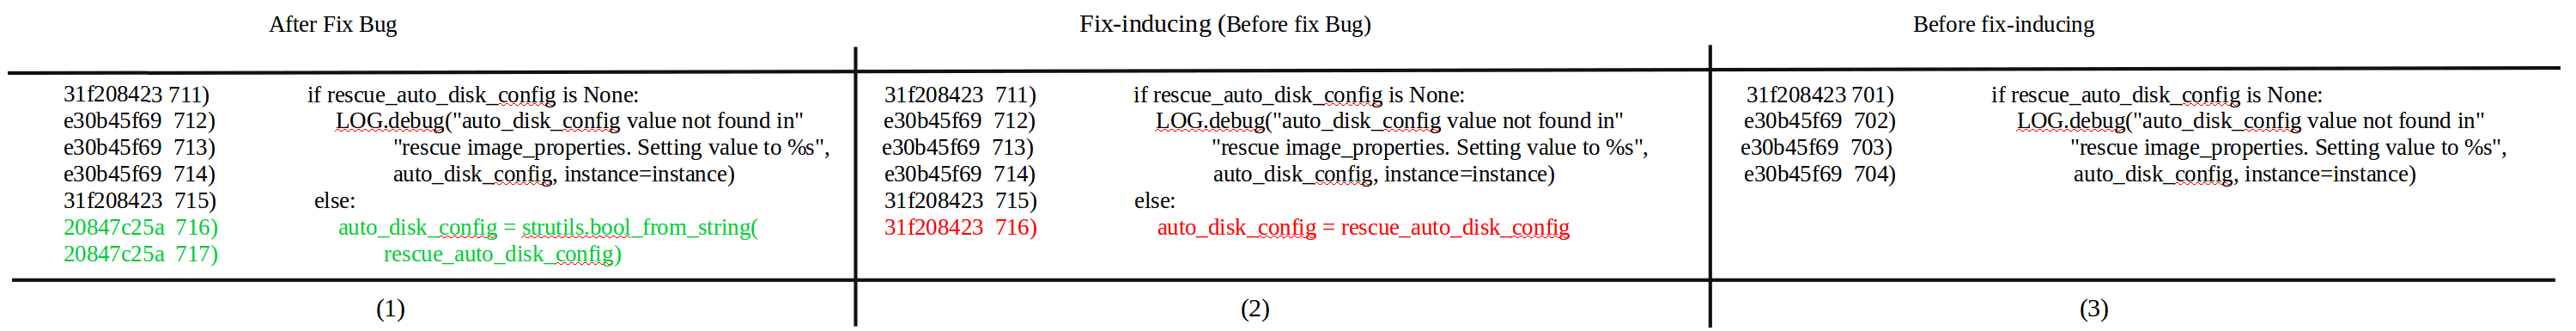
\includegraphics[height=2in, width=7in]{responsible.png}
\caption{Example of a change in which the bug was introduced in the previous commit. More recent versions of the code are on the left.}
\label{fig:1}       % Give a unique label
\end{figure*}


\begin{enumerate}
  \item The code on the left (subfigure \textit{(1)}) is the one written to fix the bug.
  \item The code in the middle (subfigure \textit{(2)}) shows the moment in which the bug was introduced (being \textit{31f08423} the id of change), the previous commit.
  \item The code on the right (subfigure \textit{(3)}) shows how in previous versions of the file, the bug did not exist.
\end{enumerate}

\begin{figure}[ht]
\centering
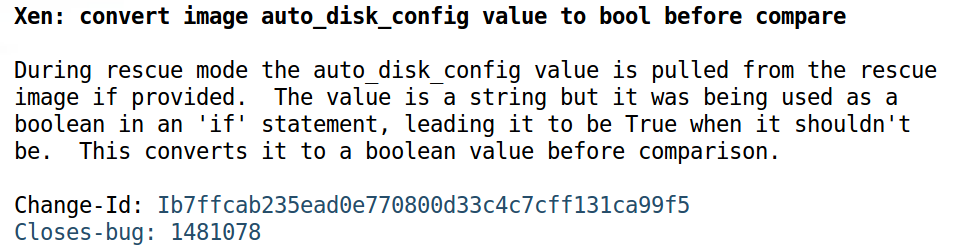
\includegraphics[height=2.4cm]{gerritPrevCommit.png}
\caption{Description of the bug-fix commit for a case in which the previous commit caused the bug.}
\label{fig:2}       % Give a unique label
\end{figure}


According to the description in the log of the commit that fixed the bug (see Figure~\ref{fig:2}), commit \textit{31f08423} was the one where the bug was introduced, as it used a string variable, while a Boolean had to be used, keeping the concordance with the rest of the code. So, in this case, the bug was introduce in the previous commit.


On the other hand, Figure~\ref{fig:3} shows a clear example of a case where the cause of the bug cannot be attributed to the previous commit. In this example, the bug fixing commit log (see Figure~\ref{fig:4}) describes that the name of an argument changed when updating the version causing the failure in the software. This change was done because of the new requirements in the software version, and is unrelated to the changes performed in the previous commit. When the modified lines where introduced the first time, they where not buggy.

\begin{figure*}[ht]
\centering
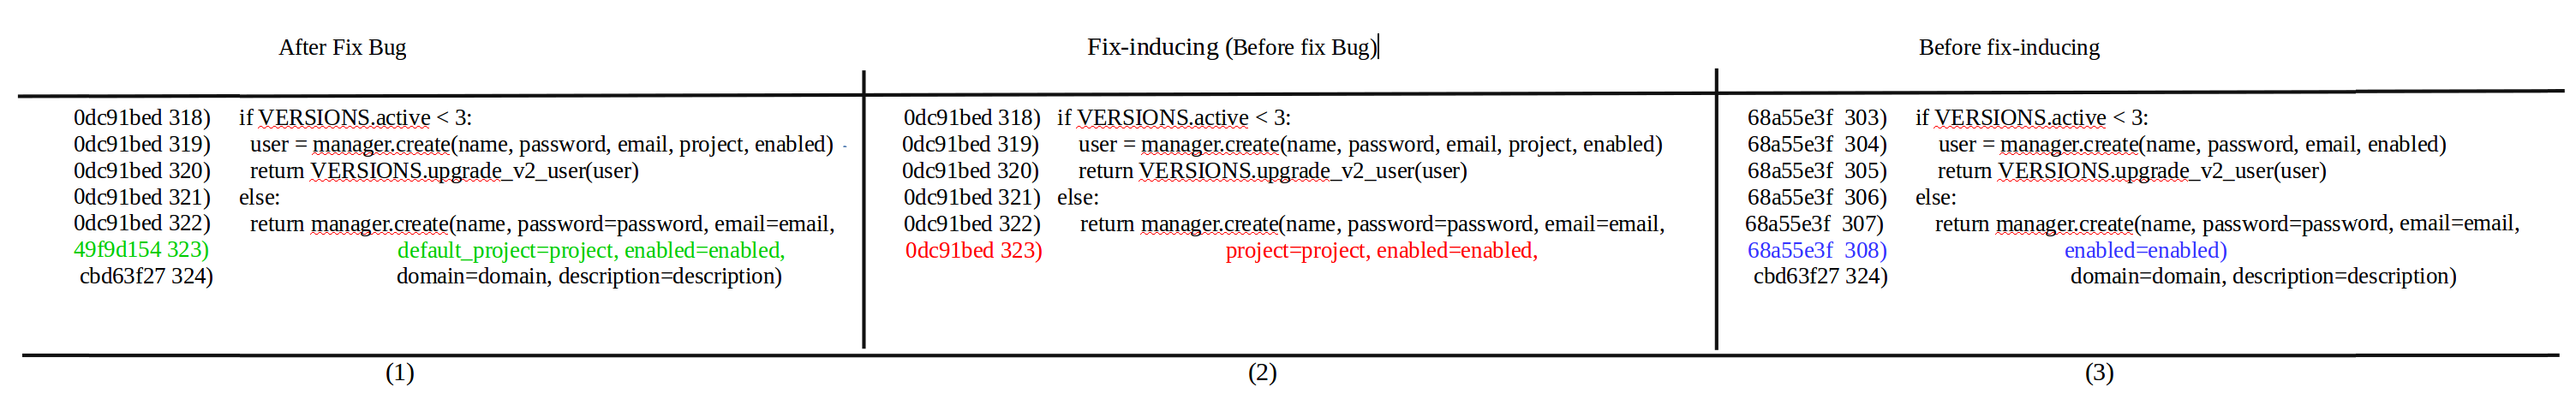
\includegraphics[height=2in, width=7in]{noResponsible.png}
\caption{Example of a change where the previous commit, 0dc91bed, did not insert the bug. More recent versions of the code are on the left.}
\label{fig:3}       % Give a unique label
\end{figure*}

\begin{figure}[ht]
\centering
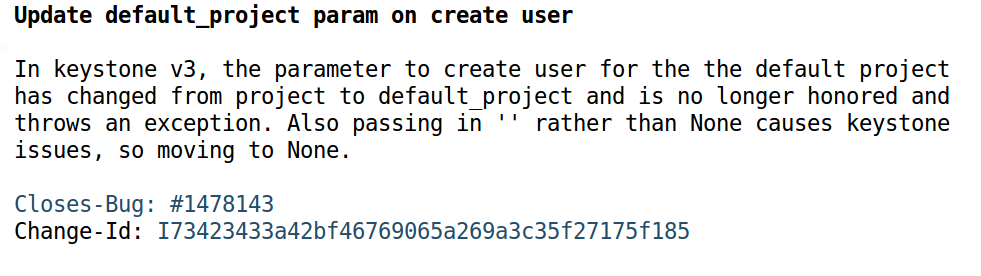
\includegraphics[height=2.4cm]{UpdateFixBug.png}
\caption{Description of the bug-fix commit for a case in which the previous commit did not cause the bug.}
\label{fig:4}       % Give a unique label
\end{figure}

Based on anecdotal evidence like the one presented in Figures~\ref{fig:3} and Figure~\ref{fig:4}, we argue that in projects that are continuously evolving, with a large development community, code that at some point was correct could become buggy later. Changes in other parts
of the code may trigger wrong behavior (bugs) in places which were correct in the past. This happens often in situations like changes of the API. In the moment the code was written, it was correct and the woftware worked fine. Additions of new features or enhancements to the API may have as a side effect that the formerly correct code starts to show a wrong behavior, making the software fail. In such cases, the source of the error cannot be attributed to the changes performed in the previous commit, which were correct when they were introduced, since in that moment they referred to a different API.

The goal of this paper is to find out to which extent the cause of bugs can be attributed to the previous commit. We will consider that the previous commit is ``responsible'' for the bug if that code was buggy (caused the malfunction) in the context of the code at the moment it was introduced. If the code was right at that time, but the bug is due to some other change in the chain of previous commits, ot to changes to other areas of the code (such as a change in APIs), we don't consider that change to be responsible of the bug.

In detail, we attempt to address the following research questions:

%\grex{rephrase RQs}
\begin{itemize}
     \item RQ1: How can we identify changes done to fix a bug?
     \item RQ2: How often is the previous commit the cause of the bug?
\end{itemize}
     
RQ2 is the main question that we want to answer in this paper: given bugs that have been fixed by changing some code, how many of those were introduced by the previous commit.
    %\item RQ1 : How can tickets which are bug reports be differentiated from those that are not?
    %\item RQ1:  How can we know that a change was done to fix a bug in the source code? How can we identify them?

But be able to answer RQ2, we first need to study the issue-tracking system and identify the subset of closed tickets that correspond to fixed bugs. In essence, RQ1 could be also stated as \emph{Which tickets in the issue tracking system are (real) bug reports?}. This is because (real) bugs are managed in an issue-tracking system together with feature requests, optimizations, test cases, etc. As we are only interested in  bugs, we need to identify those as a previous step to analyze if they have been caused by the previous commit. 

One interesting aspect of our study is that it addresses a very fundamental aspect of many studies on how bugs are fixed: the underlying assumption that there must be a commit previous to the fix, touching the same lines that were later fixed, when somebody introduced the bug. If some evidence is found that in a large fraction of the cases the corresponding code was correct when it was introduced, there is no reason to blame it as the cause of the bug, even when chenging it fixes the bug. Therefore, any result obtained after this assumption should be revisited with some care. We want to contribute with a first step in removing this uncertainty.

The remainder of this paper is structured as follows. Next, we present the current body of knowledge in section~\ref{sec:related}. Section~\ref{sec:methodology} describes the methodology used to identify the moment in which the bug was introduced in the source code, followed by the results obtained after applying our approach to a selection of OpenStack bug fixes in Section~\ref{sec:results}. Section~\ref{sec:discussion} answers the research questions and discusses potential applications and improvements of our approach. After reporting the limitations and threats to validity in Section~\ref{sec:threats}, we draw some conclusions and point out some potential future work in Section~\ref{sec:conclusions}.


\section{Related Work}
\label{sec:related}

The first algorithm to identifying bug-introducing code changes automatically was proposed by Sliwersky et al.~\cite{sliwerski2005changes}. Currently, it is a well-known algorithm called SZZ, which is based on text differences to discover modified, added and deleted lines between the bug-fix and its previous version. The SZZ algorightm uses the CVS \texttt{annotate} command\footnote{Other versioning systems provide similar functionality to CVS \texttt{anotate}; for instance, git offers \texttt{blame}.} to identify the last commit that touched these lines.

An improvement to the SZZ algorithm is described by Kim et al.~\cite{kim2006automatic}. There the authors used annotation graphs instead of CVS annotation to locate, in the previous versions, the lines affected by modification and deletion. Also, they avoid some false positives by not considering blank spaces, changes in the format or changes in the comments.

Sinha et al. present another technique to identify the origins of a bug in~\cite{sinha2010buginnings}. Their technique is not text-based technique, as the SZZ algorithm, the authors analyze the effects of bug-fix changes on program dependencies. So, taking into account the semantics of the source code they achieved higher accuracy in identifying the origins of a bug.

The two approaches have some metodological patterns in common:

\begin{enumerate}
  \item They find the differences between the bug-fix version and the previous version of the file to recognize those changes done by the bug-fix commit. 
  \item They look back in the code revision history until they identify which version touched the lines affected in the bug-fix for the last time.
\end{enumerate}

Williams et al. revisited the SZZ algorithm to track bug-inducing changes and identify types of changes~\cite{williams2008szz}. Yang et al. applied SZZ to find what kind of bug-inducing changes are likely to become a great threat after being mared as bug-fix changes~\cite{yangbug}.
Finally, some bug prediction algorithms are based on SZZ; Kim et al. showed how to classify file changes as buggy or clean using change information features and source code terms~\cite{kim2008classifying}. \grex{Creo que deberiamos hablar de mas papers que hacen uso de SZZ y derivados}. 

The SZZ algorithm (and its \emph{successors}) have had a considerable impact in the research community. Noteworthy is the fact that the paper with original the SZZ algorithm~\cite{sliwerski2005changes} has been cited, according to Google Scholar, 463 times as of January 
2016. An enhanced version of the SZZ algorithm~\cite{kim2006automatic} counts with 123 citations.


The SZZ algorithm (and its \emph{successors}) have been widely used in the research community.
Williams et al. revisited the SZZ algorithm to track bug-inducing changes and identify types of changes~\cite{williams2008szz}. Yang et al. applied SZZ to find what kind of bug-inducing changes are likely to become a great threat after being mared as bug-fix changes
Finally, some bug prediction algorithms are based on SZZ; Kim et al. showed how to classify file changes as buggy or clean using change information features and sour code terms~\cite{kim2008classifying}.

%\grex{maybe talk about my paper with dmg and ahmed, where bugs could be found elsewhere~\cite{german2009change}. There the talk is precisely about those bugs whose origina are elsewhere. Title of the paper: \emph{Change impact graphs: Determining the impact of prior codechanges}}\gema{me parece bien, no lo he leido pero nadie mejor que tu para resumirlo en esta seccion}

In the research literature, we can already find methods that consider other sources of information than the previous commit. In fact, German et al.~\cite{german2009change} 
point out that software is in constant change, and that changes performed may have impact across the whole system and may lead to the manifestation of bugs in unchanged parts. In this case, a bug emerges in a different location from the source of the bug, which is a change to a function somewhere else in the source code base. \grex{Quizas mirar si hay mas articulos en esta linea. No es muy importante esto.}


%In addition some tools are based on SZZ too such as \cite{} 
%Finally our idea.

\section{Methodology}
\label{sec:methodology}
%We present our approach to identify how and where a bug was inserted into the source code, causing a later fix. 

All data needed to analyze when the bug was introduced can be obtained from the issue tracking systems and the code review systems used generally by free/open source software (FOSS) projects. In our analysis, we have focused on Launchpad\footnote{\url{https://launchpad.net/}} as issue tracking system, and Gerrit\footnote{\url{https://www.gerritcodereview.com/}} as code review supporting tool, as they are widely used by FOSS projects nowadays, but our methodology should be generalizable to any such tool.

The Launchpad of each project works with issue reports called tickets, which describe bug reports, feature requests, maintenance tickets, and even design discussions. In our study, however, we are only interested in those tickets that have following properties:

\begin{enumerate}
  \item They describe a bug report, and
  \item They have been closed and merged in the code source to fix the described bug.
\end{enumerate}

In these bug reports we can find a comment with the link to Gerrit where the bug was fixed. It is in Gerrit where we can see all the patchsets proposed and the comments done by the reviewers. 

\subsection{Fist Stage: Filtering}
\label{sec:firstStage}

First, we have to identify what issues found in Launchpad are bug reports. This is not a trivial task and is labour intensive as it has to be done manually. As the process is repetitive, we developed a web-based tool\footnote{\url{bugtracking.libresoft.es}} that helps in the classification process. This tool offers all relevant information required to decide if an issue corresponds to a bug report or not. The tool uses information extracted automatically from the project repositories, and offers a web-based interface which allows for collaboration, traceability and transparency in the identification of bug reports.

During the identification of the issues, we have to take into account the next parameters for each ticket:

\begin{itemize}
  \item The title of the issue report
  \item The description of the issue report
  \item The description of the fix commit
  \item The changes to the source code, as sometimes neither the descriptions nor the comments by developers and reviewers in the Launchpad and Gerrit of each ticket, clarified the underlying ticket.
\end{itemize}

We can see a screenshot of the web interface of the tool in Figure~\ref{fig:screenshot}. The left side is used to display the information extracted from Launchpad and Gerrit, and the right part is the one in which the researchers can write and classify the ticket into one of the three groups. Additional meta-data, such as keywords, comments and the reviewer are included in the database.

\begin{figure}[ht]
\centering
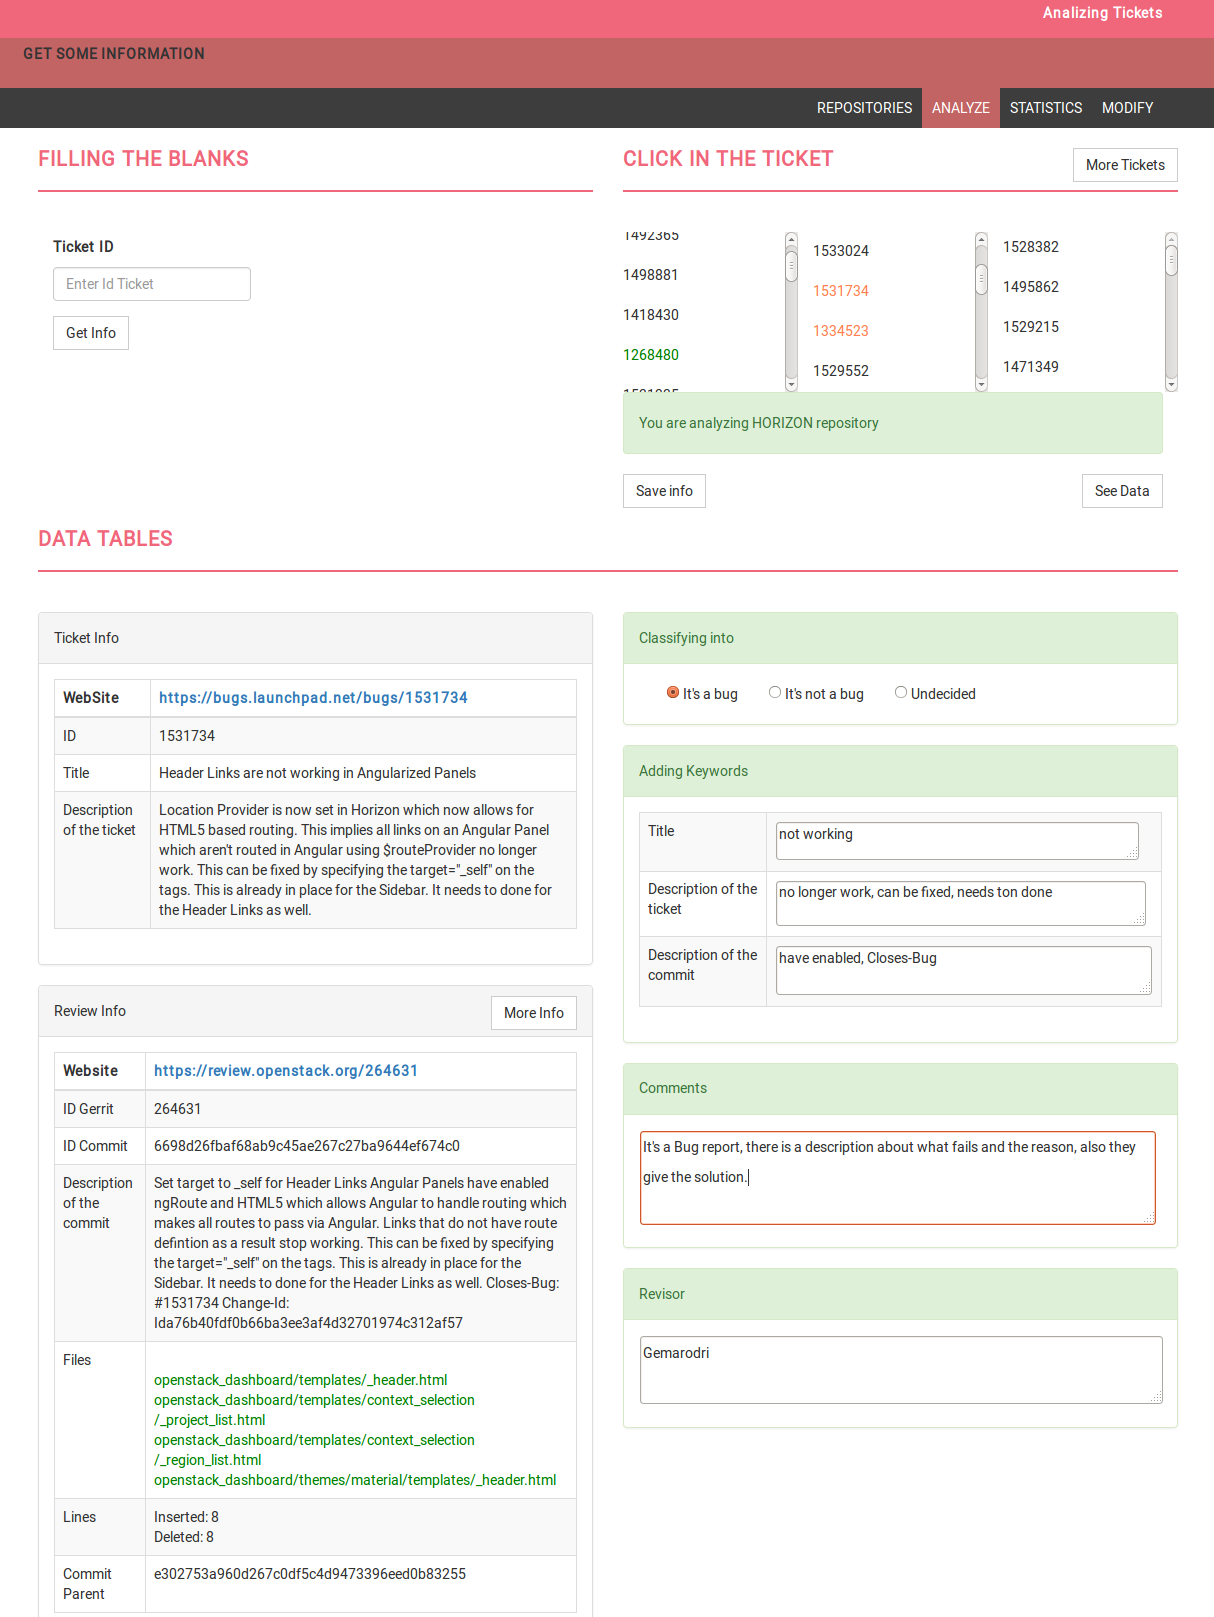
\includegraphics[height=12cm]{index.png}
\caption{Screenshot of the tool used to classify the tickets.}
\label{fig:screenshot}       % Give a unique label
\end{figure}

Each ticket was then categorized into one of three following groups:

\begin{enumerate}
  \item Group 1 (\textit{Bug Report}): The ticket describes a bug report.
  \item Group 2 (\textit{Not Bug Report}): The ticket describes a feature, an optimization code, changes in test files or other not bug reports.
  \item Group 3 (\textit{Undecided}): The ticket presents a vague description and cannot be classified without doubts.
\end{enumerate}

From the experience of analysing a small number of tickets, we agreed on following four criteria: 
\begin{enumerate}

    \item Each time that the title or the description of a ticket describes an unexpected behaviour in the program, our criteria indicated that it was considerated as a bug report. 
    \item The description of the ticket presents an optimization, deletion of a dead code or the implementation of new characteristics, we agreed not to classify it as a bug report because there is no failure. 
    \item When the ticket described that some updates were required, the ticket is a bug report. We consider all tickets that require updating as bug reports, because updating a software hints to the software not operating as expected. 
    \item When only test files are affected in a ticket, we classified it as not being a bug report. We consider bug errors in test files are a different type of bugs, as the software may still work as expected.
    
%    Test files in a ticket were not be analyzed, as we consider they are not a core part of the software and are used as a testing method to determine whether the code is fit for use. When the bug exclusively lies in a test file, the ticket was not considered as bug report because the software still works as expected, only test fails. \grex{no se repiten las frases?}\gema{Te refieres al inicio de cada frase o a lo que se describo en cada frase?}

\end{enumerate}

Sometimes we were unable to answer all the questions due to having insufficient data or because of the complexity of the issue. In this case, the ticket was classified into the \textit{Undecided} group.

\subsection{Second Stage: Who caused the Bug?}
\label{sec:secondStage}

In this second part, our work was focused on analyzing the previous commit exclusively for those tickets classified in the \textit{Bug Report} group. Therefore we had to locate the line that contained the bug, inquire the reason of the software failure, and gathering additional information on the context of the project.

For that, we had to analyze the lines involved in the bug fix and in the \emph{parent} commit of the bug fix commit, being sure that the lines were added, inserted or modified in the previous commit. We refer to \emph{parent} commit as the commit that modified any line of code in the file before the fix-bug commit, in contrast to the \emph{previous} commit where the modified lines were the same than in the fix-bug commit. It should be noted that those lines modified in the parent commit do not have to be the ones that have been modified in the bug-fix.
Figure~\ref{fig:parentgerrit} contains a snapshot of the information provided by Gerrit, where the link to the parent commit(s) can be found, that corresponds to the bug-fix shown in~\ref{fig:1}. As can be seen, the previous commit (\textit{31f08423}) in Figure~\ref{fig:1} is different from the parent commit displayed in Figure~\ref{fig:parentgerrit} (\textit{db7fc59ebc}).


We do this process to be sure that we are looking the correct change, because sometimes although the commit added many lines, if you look the code before the commit you can check that some of the lines added was there, and in that case, it is a false positive where the previous commit did not cause the bug. 


%\grex{Gema, puedes aclarar este parrafo? Que es el "parent" commit? Es lo mismo que el previous commit? Es la primera vez que hablamos de el. Quizas sea buena idea que lo reformules en castellano, porque ahora mismo es criptico}\gema{el parent commit es el ultimo commit que se hizo en el fichero antes de que se realizase el que arreglo el error, por tanto lo que hago usar diff y blame en el commit parent y en el commit que arregla el error para saber que lineas se han cambiado y que commit las cambio), y despues hago lo mismo con el commit previo y el commit parent del previo para saber que en realidad en ese momento se produjo el cambio. En el gerrit nos dan esa info como se puede ver en la figura}

%\grex{Sigue sin quedarme clara cual es la relacion entre el parent commit y el previous commit (mira que yo pensaba que eran lo mismo)... podriamos dar una definicion?}  
%\gema{EL parent commit es el ultimo commit que toco alguna linea del fichero antes de que se realizase el fix bug commit, pero las lineas que toco el commit parent no tienen porque contener ningun bug. Mientras que el commit previo es la ultima modificacion que se hizo en aquellas lineas que ha tocado el bug-fix.Estaría bien dar una definicion por si no se ve claro}

\begin{figure}[ht]
\centering
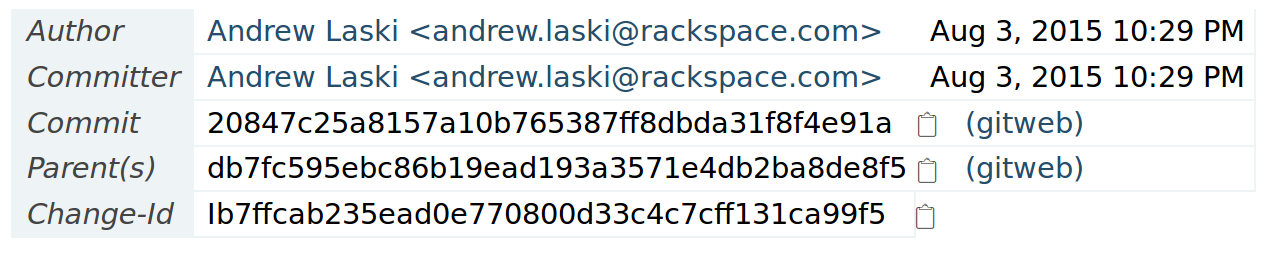
\includegraphics[height=2cm]{parent.png}
\caption{Information about the bug as displayed by Gerrit.}
\label{fig:parentgerrit}       % Give a unique label
\end{figure}


The analysis was done manually. We used \textit{git blame} to see the previous commit for each line of the involved file. Also, we used \textit{diff} to see the differences between the two files, in our case as the file is going to be the same, between the file in two different moments in the control version system.

The procedure for each file involved in a bug fix is as follows:

\begin{enumerate}
  \item git checkout \textit{commit that fixed the bug}, git blame \textit{file involved}. In this step we can see the lines added, modified or deleted by the commit that fixed the bug.
  \item git checkout \textit{parent of commit that fix the bug}, git blame \textit{file involved}. In this step we can see the previous commits for the different lines touched in the fixed bug.
  \item git checkout \textit{parent of previous commit}, git blame \textit{file involved}. With this step we can ensure that the previous commit inserted these lines.
\end{enumerate}

Finally we need to discard some noise presents in our final results according to the responsibility of the previous commit inserting the bug in the code source. Due to they were not responsible for cause the bug, we delete those previous commit which presents the following criteria:

\begin{itemize}
    \item Blank lines
    \item Format changes
    \item Copied lines
    \item Changes in the comment.
    \item Updates in the version of a file. 
\end{itemize}


\section{Evaluation}
\label{sec:evaluation}

We have validated our methodology analyzing tickets from OpenStack. OpenStack is a cloud computing platform with a huge developing community (more than 5,000 developers) and significant industrial support from several major companies such as Red Hat, Intel, IBM, HP, etc. OpenStack was particularly of interest because of its continuously evolving due to its very active community. Currently it has more than 233,000 commits with more than 2 million lines of code \footnote{\url{http://activity.openstack.org/dash/browser/}}. All its history is saved and available in a version control system, as well as its issue tracking system (Launchpad\footnote{\url{https://launchpad.net/openstack}}) and the source code review system (Gerrit\footnote{\url{https://review.openstack.org/}}).

OpenStack is composed by 9 projects, but we only focused on the main four of them: Nova, Cinder, Neutron and Horizon. As can be seen from Table~\ref{tab:OpenStack}, these projects have been very active during their entier history, and in the last year.

\begin{table}[htb]
\centering
%\begin{center} {\footnotesize
\begin{tabular}{lrr}
\toprule[0.3mm]%{\smallskip}
  & All History  & Last Year (2015) \\\hline
Nova    \kern 1pc & 14,558 & 3,283 \\
Fuel    \kern 1pc & 9,139 & 5,123 \\
Neutron  \kern 1pc & 8,452 & 3,855 \\
Horizon \kern 1pc & 4,871 & 1,994 \\
Cinder  \kern 1pc & 4,556 & 1,832 \\
Keystone\kern 1pc & 4,874 & 1,795  \\
Heat    \kern 1pc & 6,395 & 2,372  \\
Glance  \kern 1pc & 2,651 & 723 \\
Tempest \kern 1pc & 4,141 & 1,312 \\
\bottomrule[0.3mm]
\end{tabular} %}
\caption{ Commits per Project in OpenStack}
\label{tab:OpenStack}

%\end{center}
\end{table}

For these four projects we analyzed if bug fixes where introduce in their previous commits. For the first stage, we used the tool described in~\ref{sec:firstStage}. Each ticket was analyzed by two researchers independently. The second stage was done manually by the first author. %that, we extract a total of 459 tickets from this projects, in which we should be sure that the bug fixes come from a bug report, because two of five issues are misclassified \cite{herzig2013s} and this should cause bias in our final results.

\section{Results}
\label{sec:results}

A total of 459 different tickets from the Launchpad of the four main projects in OpenStack: 125 tickets from Nova, 125 tickets from cinder, 125 tickets from Horizon and 84 tickets from Neutron.

\subsection{Fist Stage}
\label{sec:resultsFS}

We classify a total of 459 tickets using the tool, resulting in 917 reviews. Only those tickets classified as bug reports by both researchers were considered in the next stage, which analyzes if the cause of the bug was introduced in their previous commits. This process requires manual inspection by researchers. In the mean classifying a ticket takes between 5 and 10 minutes per ticket, although the amount of time decreases with experience as could be expected. 

\gema{[...] se podria medir en github en tiempo que les ha llevado a cada uno entre ticket y ticket, en aquellos casos que se puedan medir y hacer una media, Que te parece?} \grex{No es muy importante, pero quedaria bien}


\begin{table*}
\centering
%\begin{center} {\footnotesize
\begin{tabular}{l|rrr|r}
\toprule[0.3mm]%{\smallskip}
  & Bug Report & Not Bug Report & Undecided & Total \\\hline
R1  & (184) 55\% & (115) 34\% & (35) 11\% & 334 (100\%) \\
R2  & (188) 76\% & (54) 22\% & (7) ~3\% & 249 (100\%) \\
R3 & (188) 56\% & (116) 35\% & (30) ~9\% & 334 (100\%) \\ \hline
Agree & (209) 72\% & (74) 25\% & (9) ~3\% & 292 (100\%) \\
\bottomrule[0.3mm]
\end{tabular} %}
\caption{Statistics for each researcher as a result of the classification process. For each researcher R, the number of tickets (and percentages) classified into the three groups is given. The \emph{Agree} row gives the number of tickets (and percentages) where two researchers agreed.}
\label{tab:2}
%\end{center}
\end{table*}

%\grex{Tiene sentido añadir porcentajes, como he hecho a la columna de Total?}
%26-56 hours

Table~\ref{tab:2} shows the classification percentages for each researcher after analyzing the tickets, and the number of tickets classified by two different researchers in the same group. %Obtaining that the researchers R1 and R2 had a similar data in their results, whereas research R2 got results significantly different with a higher number of tickets classified as Bug Report.
As a result, researchers identified 292 tickets in the same group, that is, their results matched in over 70\% of the cases. Of those, 209 tickets had been classified in the \emph{Bug report} group, 74 in the \emph{Not Bug Report} group and 9 tickets classified in the \emph{Undecided} group.

We also measured the concordance in the classification of each developer according to the project analyzed (see table~\ref{tab:3}). Values obtained by the three researchers are very similar, in general around a 70\%. The concordance values were always above 60\%. 

\begin{table*}[htb]
\begin{center} {\footnotesize
\begin{tabular}{l|rrrr|r}
\toprule[0.3mm]%{\smallskip}
  & Nova & Cinder & Horizon & Neutron & Total\\\hline
R1 -- R2   & (44) 70\% & (40) ~77\%  & (37) 60\% & -        & (121) 68\% \\
R1 -- R3   &  -        & (46) ~73\%  & (48) 76\% & (26) 62\% & (120) 71\% \\
R2 -- R3   & (41) 66\% & (10) 100\% & -         & -        &  (51) 71\% \\
\bottomrule[0.3mm]
\end{tabular} }
\caption{Concordance among researchers for each repository.}
\label{tab:3}
\end{center}
\end{table*}


After this, we can answer the first research question because at this moment we have all the data necessary and all the knowleadge to can distinguish bug reports from others reports.

\vspace{0.2cm}
\fbox{\begin{minipage}{25em}
\textbf{RQ1: Using all the information available in the bug tracking system and code review systems related to a bug-fix, we have obtained that in at least 72\% of the tickets analyzed the bug-fixs were real bug reports.} 
\end{minipage}}
\vspace{0.1cm}


\subsection{Second Stage}
\label{sec:resultsSS}

In this stage we analyzed the 189 tickets of the classified as \textit{Bug Reports}, the possible outcome of the analysis was one of the following three options:

\begin{itemize}
  \item Cause
  \item No Cause
  \item Undecided
\end{itemize}

This analysis takes into account that the bug could span many lines that may belong to several previous commits, but in fact, not all of them could had caused the bug. It may happen that in the previous commit, lines have been copied from further previous commits, comments may have been modified or blank spaces/lines have been introduced. Hence, the cause could be found in a single previous commit, in many or even in none. 

Figure~\ref{fig:manyprevious} contains a real example of a previous commit where more than one commit has been identified. In this case, we have two possible commits: \textit{e7be0a988} and \textit{e5296c1da}. Previous commit \textit{e7be0a988} did not cause the bug, because the modification affects only the version number of the software. It is previous commit \textit{e5296c1da} the one that caused the bug, because it introduced an incorrect \texttt{break} line. %\grex{Todavia no esta del todo claro... yo creo que esto merece un ejemplo - incluso con codigo real, tal y como hemos hecho al principio del articulo. Ademas, nos lo podemos permitir; tenemos espacio.}\gema{perfecto, ahora busco un ejemplo y lo anado abajo}

\grex{No estan mal las descripciones superiores en la figura~\ref{fig:manyprevious} que dice ``After Fix Bug'' y ``Fix-inducing (Before fix bug)''?}
\gema{creo que no, la de la izquierda es despues de que se arreglara el error, y la de la derecha es en el momento en que se introdujo el error}
\begin{figure}[ht]
\centering
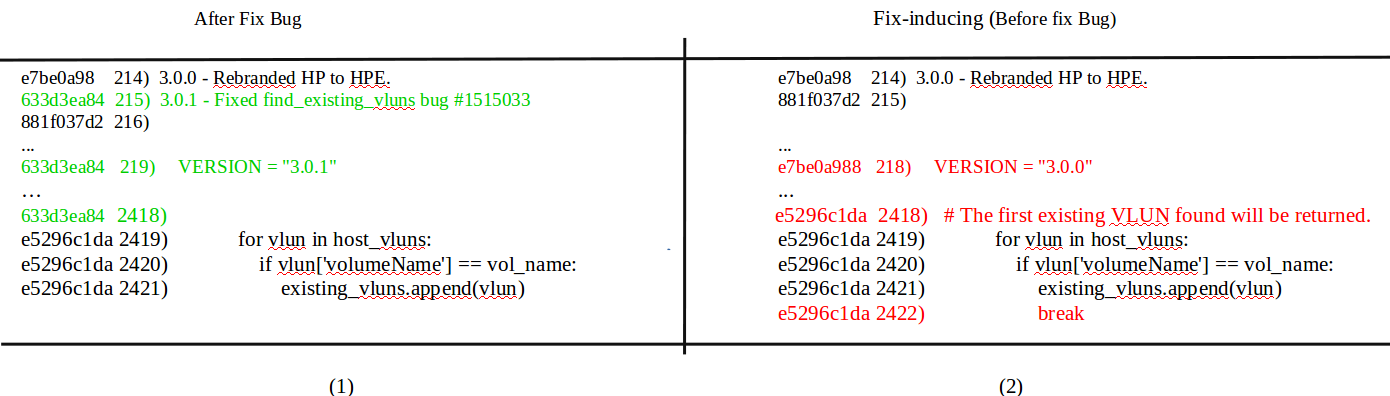
\includegraphics[height=2.5cm]{manyprevious.png}
\caption{Previous commits (right): \textit{e7be0a988} (line 218) and \textit{e5296c1da} (line 2422).}
\label{fig:manyprevious}       % Give a unique label
\end{figure}


We identified a total of 348 previous commits which could be the cause of the 189 bug reports under analysis. Then, we analyzed the bug reports together with their previous commits discarting the cases where the previous commit was a false positive (blank lines, changes in comments or even a change in the version of the file). So, in total we have analyzed 308 previous commit.

As can be seen in Table~\ref{tab:responsability}, from the 308 previous commits, 152 have been considered to be the cause of the bug, whereas 114 were identified as not beign the cause. We were unable to decide in 42 cases or due to our limited knowleadge about the code. The figure \ref{fig:add} shows the change done in the fix bug commit, on the left the lines before the fix commit and on the right the file after the fix commit with only additions lines. In this case, we cannot be able to know which previous commit could be the one that forgot added this lines, this is the reason why we classifyed as \textit{Undecied},\grex{Gema, puedes poner un ejemplo de estas dos cosas? Uno de solo added lines y otro de limited knowledge. Si el ejemplo es verdadero, mejor.}\gema{Me faltaria el ejemplo de limited knowledge, cuando encuentre uno bueno lo anado}
We discarded 40 more because they were false positives (\emph{noise}) such as blank lines, changes in comments or even a change in the version of the file.
\begin{figure}[ht]
\centering
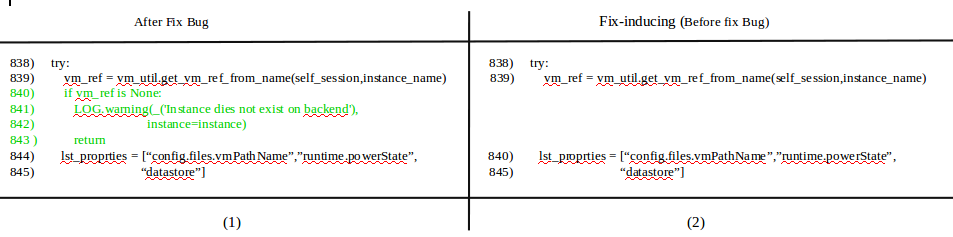
\includegraphics[height=1cm]{addedlines.png}
\label{fig:added}       % Give a unique label
\caption{Example of added lines where we are unable to decide which previous commit caused the bug}
%52919
\end{figure}

%\begin{figure}[ht]
%\centering
%\includegraphics[height=2cm]{unknown.png}
%\label{fig:9}       % Give a unique label
%\caption{Example of unknowleadge where we are unable to decide which previous commit caused the bug }
%\end{figure}
\begin{table}[htb]
\begin{center}
\begin{tabular}{lrr}
\toprule[0.3mm]
  & \multicolumn{1}{c}{Before} & \multicolumn{1}{c}{After} \\
  & \multicolumn{1}{c}{Deleting Noise} & \multicolumn{1}{c}{Deleting Noise} \\\hline
{Cause} & (152) 44\% & (152) 49\% \\[0ex]
{Not Cause} & (154) 44\% & (114) 37\% \\[0ex]
{Undecided} & (42) 12\% & (42) 14\% \\[0ex]
\bottomrule[0.3mm]
\end{tabular}
\caption{Number of times (and percentage) where the previous commit is the cause, not the cause or could not be classified, before and after deleting noise.}
\label{tab:responsability}
\end{center}
\end{table}


If we attend to how many previous commits each of the 189 bug reports analyzed had, we see that 131 only had a previous commit as the example \ref{fig:3}, whereas 58 had more than one previous commit as the one shows in ~\ref{fig:manyprevious}. In Table~\ref{tab:secondStage}, from the 131 unique previous commits, 65 were the cause of the bug, and 30 not caused the failure. For the 58 bugs that had more than one previous commit, a total number of 179 previous commits were identified; of them 86 were the cause of the bug, while 82 were not. \grex{Pon ejemplos, a ser posible reales, de esto, porfa.}\gema{perfecto, ahora busco un ejemplo y lo anado abajo}

\grex{No me queda claro que quieres decir con mas de un identificador previo}\gema{supongo que despues de ver el ejemplo se entienda mejor, identificador previo se refiere a que  al arreglar el error se shan tocado varias lineas que han sido anadidas o modificadas en commit diferentes, por tanto tenemos mas de un commit diferente, aqui use identificador en vez de commit y puede ser un error}

\grex{Para los 58 bugs que tenian mas de un identificador previo hay 179 commits. Bien. Dices que 86 causaron el bug, 82 no y en 11 no se ha podido determinar. Lo que no veo es por que no agruampos estos datos segun los 58 bugs}\gema{Esos datos estan agrupados en la tabla 7, el fin de esta tabla era mostrar que cuando hay un solo comit previo el numero de no causantes del error es menor que cuando hay mas de un commit previo}

% Furthermore, focusing on how many previous commits presented each Bug Report, we obtained that 131 had one previous commit implicated, whereas 58 had more than one previous commit implicated in their file/s. According to Table \ref{tab:secondStage}, from the 131, we obtained that 65 of them inserted the bug, but 30 of them were not responsible in the failure of the system. And from the 58 which had more than one previous commits, we obtained in total 189 previous commit, where 86 of them were responsible and 82 were not responsible. %Probably, the bug was inserted in different lines of different commits, but not everyone has to be responsible for the commit, sometimes the previous commit copied lines from its previous commit or inserted comments and blank spaces. After the analysis the responsible can be only one of them, more than one or maybe none. 

\begin{table}[htb]
\begin{center} {\footnotesize
\begin{tabular}{lcc}
\toprule[0.3mm]
  & \multicolumn{1}{c}{One previous } & \multicolumn{1}{c}{More than one previous} \\
  & \multicolumn{1}{c}{commit} & \multicolumn{1}{c}{commit} \\\hline
\raisebox{1ex}{Cause}     & (65) 50\% & (86) 48\% \\[0ex]
\raisebox{1ex}{Not cause} & (30) 23\% & (82) 46\% \\[0ex]
\raisebox{1ex}{Undecided} & (36) 27\% & (11) ~6\% \\[0ex]
\bottomrule[0.3mm]
\end{tabular} }
\caption{Probability of the cause of the bug when the bug report present one previous commit or more than one previous commit.}
\label{tab:secondStage}
\end{center}
\end{table}


%\gema{Los resultados que he obtenido y que queria plasmar en las tablas son:}
%\gema{- He analizado 189 bugs reports}\\
%\gema{- De los 189, 131 presentaban el mismo identificador de commit previo para todas las lineas que habian sido modificadas, mientras que 58 presentaban mas de un identificador de commit previo.}\\
%\gema{- Dentro de los bugs reports que tienen mas de un commit previo analizando el total de todos los commits para saber quien causo el bug, he encontrado que en total de los 179 comit previos 86 causaron el bug mientarsa que 82 no lo causaron y 11 no he podido decidir si eran causantes o no.}\\
%\gema{- Ademas he mirado como se distribuyen los commits en cada bug report dentro de cada proyecto analizado, y he visto que por ejemplo Neutron presentaba 11 bugs report con solo un ticket previo, 3 bugs report con dos identificadores diferentes para los commit previos, 2 bug reports que presentaban  3 commit previos... etc.}\\
%\gema{- Finalmente realice otra clasificacion en la que tenia en cuenta el numero de commits que fueron causantes del error para un mismo bug report. Al analizar los bug reports encontre que en aquellos que presenstaban mas de un commit previo no todos los commit eran causantes del error, y en ocasiones solamente habia un commit que causo el error y los otros no o por el contrario habia bugs report en los que ninguno de sus commits previos era responsable y otras ocasiones en las que todos los commits previos eran responsables. Por tanto la tabla 7 muestra cual es la responsabilidad (tods responsables, al menos uno ningun responsable y desconozco la responsabilidad) de los coommits previos presentes en un bug report. Por ejemplo, bugs reports que tenian dos commits previos, en 4 de ellos los dos commits previous eran responsables, mientras que en 9 bug report habia al menos un responsable y en otros 4 bug report ninguno de los dos commit previos eran responsables.}  

We also studied the distribution of the number of previous commits for each bug. This result will provide further insight into the bug-seeding nature; it offers as well an idea of the complexity of identifying the cause of a bug, as the more commits involved, the harder it is to identify the cause and understand it. As shown in Table~\ref{tab:secondStage2}, usually the number of commits that can be considered as previous is 1 (over 69\% of the cases), followed by 2 commits (13\%). In around 10\% of the cases, 3 or more commits are involved.

% the number of commits that can be considered as previous is 1, followed by 2 commits. \grex{the number of commits that can be considered as previous is 1, followed by 2 commits. No se que queremos decir} \grex{Tenemos que responder a estas dos preguntas todavia: Por que es interesante hacer lo que se comenta en este parrafo? Que utilidad tiene?}\gema{Creo que era interesante saber como se distribuyen los causantes de los bugs en cada projecto y cuantos commits previos presentan los bugs report en cada projecto analizado, ademas cuantos mas commits previos, en ocasiones, es muy dificil saber quien es el responsable por tanto pense que podria haber algun patron en relacion con el numero de commits previos y cuantos de ellos son responsables, pero parece que esto no ocurre con la muestra que hemos analizado.}

\begin{table*}[htb]
\begin{center} {\footnotesize
\begin{tabular}{lccccc}
\toprule[0.3mm]
  & \multicolumn{1}{c}{One previous} & \multicolumn{1}{c}{two previous} & \multicolumn{1}{c}{three previous} & \multicolumn{1}{c}{four previous} & \multicolumn{1}{c}{+five previous}\\
  & \multicolumn{1}{c}{commit} & \multicolumn{1}{c}{commit} & \multicolumn{1}{c}{commit}& \multicolumn{1}{c}{commit}& \multicolumn{1}{c}{commit}\\\hline
\raisebox{1ex}{Neutron} & 11 & 3 & 2 & 2 & 0 \\[0ex]
\raisebox{1ex}{Horizon} & 39 & 8 & 3 & 2 & 4 \\[0ex]
\raisebox{1ex}{Nova} & 44 & 5 & 2 & 4 & 4 \\[0ex]
\raisebox{1ex}{Cinder} & 37 & 9 & 6 & 2 & 2\\[0ex]
\raisebox{1ex}{Total} & 131 & 25 & 13 & 10 & 10\\[0ex]
\bottomrule[0.3mm]
\end{tabular} }
\caption{ Distribution of the number of commits that can be considered as the previous commit per bug report for each project.}
\label{tab:secondStage2}
\end{center}
\end{table*}

Finally, we were interested in analyzing, for those cases where more than one previous commit exist, how many of them introduced the bug in the code source. Even if several previous commits are involved, it may be the case that none, at least one of them or all of them is the cause of the bug.

Results are given in Table~\ref{tab:secondStage3}; in 8 bug reports all the previous commits were identified as the cause, in 30 bug reports at least one of the previous commits caused the bug, and in 11 bug reports none of the previous commits introduced the bug. If we look at bugs that had two previous commits, in 4 cases both commits were the cause, in 9 cases only one of them was the cause and in another 4 cases non of them could be determined as the cause.

\grex{Entiendo el resultado del parrafo anterior, pero me falta una explicacion de por que esto es interesante y para que puede servir.}\gema{Para entender como de complejo es el problema, porque no es lo mismo que dos commits anteriores sean responsables a que lo sean 5, entendiendo que si son cambios independientes es muy raro que sean causantes de un mismo error. y para saber si algun patron se repite y nos ayuda a entender algo, pero las tablas no llegan a ser muy concluyentes y los numeros son bajos, podemos introducirlo como un poco de discusion sobre que podria ser interesante analizar mas y ver si con mas poblacion se repite algun patron y decir exactamente cuantos comits son los responsables en un bug report.}

\begin{table*}[htb]
\begin{center} {\footnotesize
\begin{tabular}{lccccc}
\toprule[0.3mm]
   & \multicolumn{1}{c}{two previous} & \multicolumn{1}{c}{three previous} & \multicolumn{1}{c}{four previous} & \multicolumn{1}{c}{+five previous} & \multicolumn{1}{c}{Total}\\
  & \multicolumn{1}{c}{commit} & \multicolumn{1}{c}{commit}& \multicolumn{1}{c}{commit}& \multicolumn{1}{c}{commit}\\\hline
\raisebox{1ex}{All are the cuase}          & 4 & 3 & 0 & 1 & 8\\[0ex]
\raisebox{1ex}{At least one is the cause} & 9 & 7 & 5 & 9 & 30\\[0ex]
\raisebox{1ex}{None is the cause}         & 4 & 2 & 4 & 1 & 11\\[0ex]
\raisebox{1ex}{Undecided}                & 1 & 0 & 1 & 0 & 2\\[0ex]
\bottomrule[0.3mm]
\end{tabular} }
\caption{Number of previous commits identified as the cause of a bug per bug report}
\label{tab:secondStage3}
\end{center}
\end{table*}


\vspace{0.2cm}
\fbox{\begin{minipage}{25em}
\textbf{RQ2: Only 50\% of the previous commits analyzed caused the failure in the system, whereas the 37\% of them did not introduce the bug in the code source.} 
\end{minipage}}
\vspace{0.1cm}


\section{Discussion}
\label{sec:discussion}

The experience gained in this study with exposure to several hundreds of bugs allows us to state that determining who (or what) introduced a bug is a non-trivial task.

Although at first, as shown in the Figure~\ref{fig:1} and Figure~\ref{fig:2}, one may think that this is an easy task, we have found many examples where we have been unable to determine the cause as no previous commit can be identified. This is, for instance, the case when only code has been added and there is no way to identify the previous commit. In this case, further research could find out if this is not really the addition of a new feature rather than a bug.

And we are talking about a bug report not a new feature, these kinds of cases use to be when a researcher forgot check some case inside a function.
\begin{enumerate}
\item Is responsible the function where these lines are content?
\item Is responsible the last commit that modify something in the function?
\end{enumerate}

\grex{Puedes elaborar un poco mas el parrafo (y los puntos) anterior(es)? Puede ser en castellano.}
\gema{En casos de que el error se arregle solamente anadiendo lineas, al intentar saber quien es el causante, podemos pensar en que el responsable podria ser el primero que introduce la funcion que olvido tener en cuenta ese caso, o si la funcion en la que se anade el codigo ha sido modificada varias veces pordriamos pensar que el ultimo que modifico la funcion puede ser el causante porue no se dio cuenta que fataba por anadir ese codigo. Otro caso puede ser lo if/else, en estos casos hay que ser cuidadosos y saber diferenciar si el causante fue el comit previo porque se olvido de comporbar una condicion, o si el commit previo no fue el causante del error porque la condicion que se introduce en el commit que arregla el error se debe a que han anadido una nueva funcionalidad despues de haber anadido el if/else y necesitan comprobarla ahora, por tanto seria debido a la evolucion del projecto. En este ultimo caso, si no tenemos toda la descripcion de lo que realmente esta pasando, para poder decidir en que situacion estamos, hemos sido conservadores y hemos inducado que el commit anterior fue el responsable}

There are other cases where it is difficult to determine if the change is the cause. For instance, when additional conditions are added to \emph{if}s or \emph{else}s, one might think that in the previous commit those were not included due to an error, so that the previous commit becomes the cause of the bug. However, situations exist where the additional conditions in an if appear because of the introduction of a new functionality, and thus the line in the previous commit was correct at the time it was introduced. In our analysis, if the latter situation is not explicity mentioned we have considered that the previous commit caused the error.

But already the identification of an issue as a bug report is a process that is not as straightforward as one might think. Out of 459 tickets we were only capable to achieve a consensus for 292 cases (63.6\%), which hints to the complexity of the task. The amount of information, the number of fields and the requirement of human interaction made us invest time in the creation of a tool that assisted us in the process. 


%\begin{enumerate}
% \item No todos los casos son tan claros como los mostrados en los ejemplos, hay ocasiones en las que solo se ha anadido codigo y no somos capaces de encontrar al responsable por que no existe ninguna manera de poder identificar al commit previo. 
% \item Hemos sido conservadores, en ocasiones cuando se han modificado lineas como if/else y se han anadido comprobacione que anteriormente no estaban, se puede pensar que el commit previo que toco la linea se olvido de realizar dichas comporbaciones, y en ese caso seria el causante del bug. Pero existen casos que la comprobacion que se necesita en el if ha aparecido porque se introdujo una nueva funcionalidad, por stanto en el momento original en el que se escribio la linea por primera vez no habia ningun error. Por tanto a menos que se descrisba esta ultima situacion en la descripcion del commit o del bug report, he considerado la idea treadicional, que el commit anterior provoco el error, porque realmente era dificil saberlo.
% \item Hemos utilizado la herramienta porque es un proceso complicado. Para la primera parte de decidir si es o no es un bug report hemos tenido que desarrollar la herramienta.
%\end{enumerate}

%\gema{Algunos de los problemas que nos hemos encontrado durante el analisis y que podrian ser resueltos de otra forma diferente a la nuestra y quizas puede que varie algo los resultados no lo se}

In any case, our research shows evidence that assuming that the previous commit is where the cause of a bug can be found does not hold for a not insignificant percentage of bugs. \grex{Tengo que elaborar mas esto, que es el punto mas impactante del articulo.}


\section{Threats to validity}
\label{sec:threats}

As any other empirical study, this one presents several threats to its validity, external and internal, that have to be considered and taken into account. In order to allow others to study it in detail, replicate it or even build on top of it, we have set up a replication package\footnote{\url{http://gsyc.urjc.es/~grex/repro/2016-msr-prevcommit}} including data sources, intermediate data and scripts that can be obtained.


%The limited sample size of tickets used in this research is the major threat to its validity. %It may happen, that only with 100 seemingly random tickets, there may be a prior unknown tendency. This is in fact similar to~\cite{sliwerski2005changes}, where the trend indicates that most bugs are fixed on Fridays.
The number of the tickets extracted form Launchpad is high, but probably not as high as to state that it can be representative of all free/open source systems, or the software industry. It has not to be forgotten that the analysis requires a lot of human effort, so that achieving large numbers of cases is difficult.


The internal threats related to the researchers that have conducted the study are following:

\begin{itemize}
  \item We have not considered those tickets where the two researchers showed discordance. 
%  \begin{enumerate}
%    \item Should they discuss after their analysis to reach a better classification?, Should the tool provide this?
%    \item Does the Bug report only the same ticket classified as Bug report for all the researchers?
%  \end{enumerate}
    \item We have not taken into account errors that have been classified into \textit{Undecided}, and probably we have lost some \emph{actual} bug reports.
    \item There could be some lax criteria involving the subjective opinion of the researchers.
    \item Although the researchers are experienced programmers, they are not experts in the  OpenStack project, and their inexperience may have influenced the results of the analysis.
    \item We are only using part of the information that the tickets provide, like comments and text. There could be a recognized pattern in the data, unknown at first sight, that involves other parts of the information.
    \item We have used a random script to extract the tickets from Launchpad that have been reported during 2015. There could be unintended bias of the data, because many reasons, as for instnace the phase of the project.
    \item In some cases, researchers may have classified the previous commit as the cause of the bug, even if this may not be the case (see discussion on additional conditions in if statements).
\end{itemize}

The external threats, related to the case of the project, are following:

\begin{itemize}
    \item The word \textit{bug} is continuously mentioned in the description and commit of a ticket even when we found it is not an error. This could lead to the incorrect classification during the reviewing process.
    \item Some tickets are not explicitly described, which could increase the percentage of \textit{Undecided}. This is especially true if the reviewers are not from OpenStack.
    \item OpenStack is a special project with a constant evolution due to their active community of developers. Maybe, in other projects with less commits per year, results may be totally different.
\end{itemize}


\section{Conclusions and Future Work}
\label{sec:conclusions}

The empirical experiment carried out in OpenStack supported that the current premise assumed does not hold for a large fraction of the analyzed bugs, because around the 40\% of the previous commits were not the cause of the bug.

With our methodology we have identifie which are real changes that introduced the bug, and this could be useful to improve the accuracy of those tools developed to prevent bugs. Also, the software developers stand to benefit from identifying where the bug was inserted, improving their methodology.
%How to plan to apply the knowledge in a way that can benefit software engineers.
%What are the anticipated contributions of the work?  How will you evaluate them to demonstrate usefulness?


A final field of future work could be concerned with the full automation of the methodology, developing  an automatic classifier based on the idea that not all the previous commits inject the bug. \grex{mejorar este parrafo.}

Another interesting investigation could perform the same empirical study on a project with a less active community, to prove if our idea is fulfill in other projects. So, for projects that do not evolve as rapidly as OpenStack, e.g., those with a more stable API, could offer completely different results even if applying the same analysis methodology used in this paper.


%ACKNOWLEDGMENTS are optional
\section{Acknowledgments}

We thank Dorealda Dalipaj and Nelson Sekitoleko, two PhD students in our research team, that participated in the process of classifying bug reports. We also want to express our gratitude to Bitergia\footnote{\url{http://bitergia.com/}} for the OpenStack database and the support they have provided when questions have arised. 
Finally, we would like to acknowledge the Spanish Government because all authors are funded in part by it, through project TIN2014-59400-R.

\nocite{*}
%
% The following two commands are all you need in the
% initial runs of your .tex file to
% produce the bibliography for the citations in your paper.
\bibliographystyle{abbrv}
\bibliography{sigproc}  % sigproc.bib is the name of the Bibliography in this case
% You must have a proper ".bib" file
%  and remember to run:
% latex bibtex latex latex
% to resolve all references
%
% ACM needs 'a single self-contained file'!
%
%APPENDICES are optional
%\balancecolumns
\end{document}
